%%=============================================================================
%% Technische Analyse
%%=============================================================================
\chapter{Technische Analyse}
\label{ch:technischeanalyse}

\section{Architectuur}
Voor het proof of concept zullen 3 applicaties worden gemaakt:
\begin{enumerate}
    \item D365FO applicatie met eigen model ('chtbt')
    \item C\# .NET webapplicatie voor authenticatie
    \item Implementatie in het MS Bot Framework
\end{enumerate}
\begin{figure}[h]
    \centering
    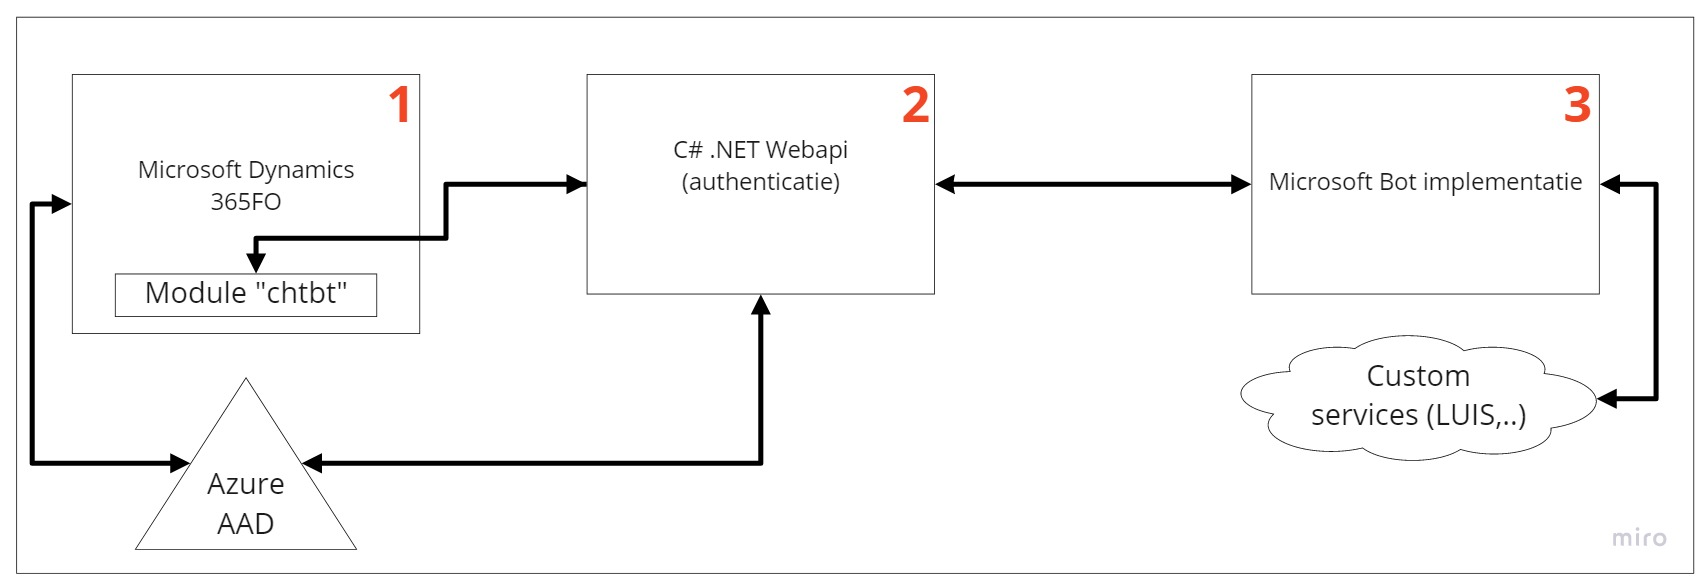
\includegraphics[width=1\textwidth]{img/ApplicatieArchitectuur}
    \caption{Applicatie architectuur}
\end{figure}
De eerste applicatie dient voor het programmeren van custom services binnen D365F0. Hiervoor zal een apart model gebouwd worden, genaamd 'chtbt' (afkorting voor chatbot). Binnen deze applicatie zal bestaande logica uit D365FO gebruikt, en beschikbaar gesteld worden d.m.v. een webservice. 

De tweede applicatie zal vervolgens connecteren met de eerste, en als communicatiemiddel dienen tussen de eerste en de derde applicatie. De reden dat hiervoor een aparte webapplicatie werd gebouwd is om de scheiding van taken en verantwoordelijkheden duidelijk af te bakenen per applicatie. Zo zal het authenticatiegedeelte (zie later) in deze omvat worden om gevoelige informatie (verbindingssleutels Azure, etc.) te verbergen voor de buitenwereld. 

Tenslotte zal uiteraard ook een chatbot gebouwd worden. Als deze dan wilt communiceren met D365FO om bepaalde CRUD-operaties uit te voeren, hoeft het enkel requests te versturen naar de authenticatie applicatie.

\section{Ontwikkel omgeving}
De ontwikkeling van het POC gebeurt volledig in de cloud, en dit op een Remote Desktop die draait op Lifecycle Services van Microsoft. Dit is een portaal waar meerdere mensen kunnen samenwerken, en dat de gebruiker assisteert in het beheren van de applicatie lifecycles van de verschillende D365FO implementaties.
Een schematische voorstelling:

\begin{figure}[H]
    \centering
    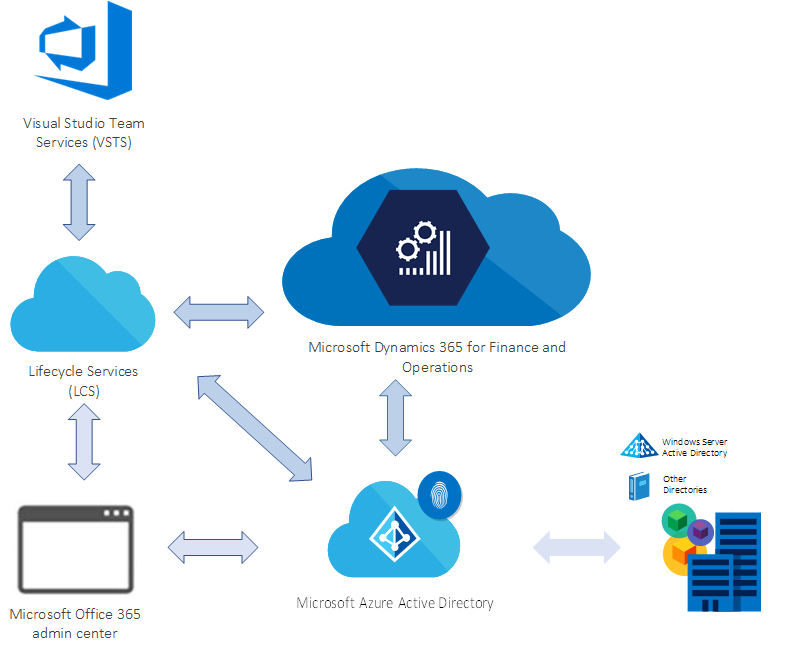
\includegraphics[width=0.8\textwidth]{img/lcsCloudArchitecture.png}
    \caption{Microsoft Lifecycle Services cloud architectuur}
\end{figure}

Aangezien dit proof of concept veel webrequests omvat, wordt er voor gekozen om deze eerst via de localhost te ontwikkelen. In een volgende stap zullen deze dan gehost worden. 

\section{Demo omgeving}
Wat betreft demo's van het poc zullen deze steeds 100\% in-cloud uitgevoerd worden. Dit wil zeggen dat alledrie de applicaties gehost zullen worden op hun respectievelijke webadressen. Enkel de bot zelf zal op de localhost runnen. 

\section{Authenticatie}
De authenticatie tussen Dynamics 365FO en de chatbot vereiste een aparte applicatie. Dit omdat de authenticatie volledig via Azure AAD verloopt. De authenticatie app werd geregistreerd binnen de D365FO Azure AAD applicaties (in D365FO: dashboard -> Azure Active Directory Applications). In D365FO ziet dit er als volgt uit: 
\begin{figure}[H]
    \centering
    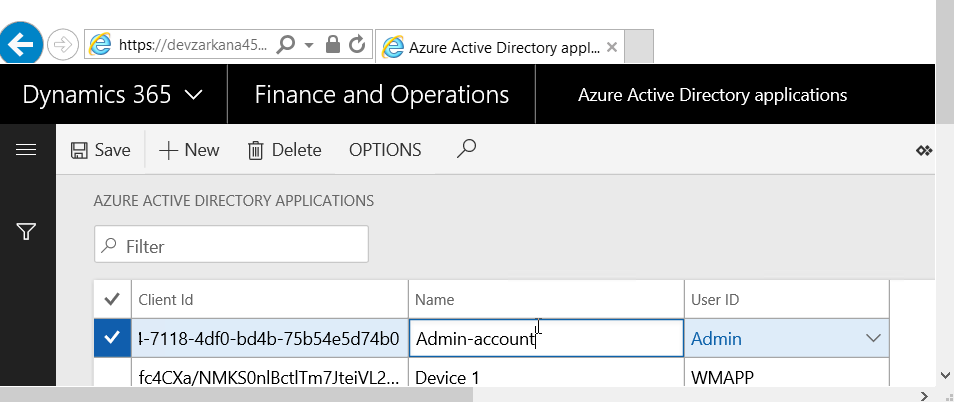
\includegraphics[width=1\textwidth]{img/impersination.png}
    \caption{Azure AAD App registrations binnen D365FO}
\end{figure}
Nadat dit gebeurd is, kan er geconnecteerd worden met D365FO van buitenaf adhv. impersonation. Een korte beschrijving van de werking: 
Wanneer iemand van buitenaf wilt inloggen op een d365FO omgeving, moet deze eerst inloggen op Azure om een Authorization Token te ontvangen. Vervolgens kan de gebruiker dan toegang aanvragen aan de resource via Azure AAD. Azure AAD zal vervolgens zo een Acces Token toekennen adhv de gebruikte credentials. 

Vervolgens kan de verkregen Acces Token gebruikt worden in requests naar D365FO. De taak van D365FO zal dan slechts zijn om deze token te controleren en verifiëren of deze nog geldig is. Hier neemt de impersonation plaats: in plaats van dat D365FO je gaat 'inloggen' adhv een username en password, zal het in dit geval anders gebeuren. Nu zal D365FO immers controleren of de Client Id (verkregen van Azure AAD) gekend is in het systeem, en zoja je inloggen met de user account geassocieerd met die Client Id. In bovenstaande afbeelding (6.3) ziet men staan dat de Client ID I-7... geassocieerd wordt met een Admin account. Met andere woorden: als D365FO een request verkrijgt met deze ID, zal het de gebruiker inloggen als admin. 


Dit proces kan ook versimpeld uitgelegd worden in volgende analogie, geschreven door Ward Lanssens (delaware); 


\begin{quotation}
    Zie het als naar de dokter gaan. Eerst controleert de dokter wie je bent (third party app doet dit bij Azure AAD). Vervolgens zeg jij wat je wil (niet gaan werken wegens ziek). De dokter geeft een briefje (token), en jij geeft dat token/briefje aan je baas (D365FO). Je baas controleert niets meer, behalve de echtheid van dat briefje. Hij gaat er van uit dat als jij dat briefje hebt, dat ondertekend is door de dokter, dat het wel zal kloppen wat je zegt.
\end{quotation}


\begin{figure}[H]
    \centering
    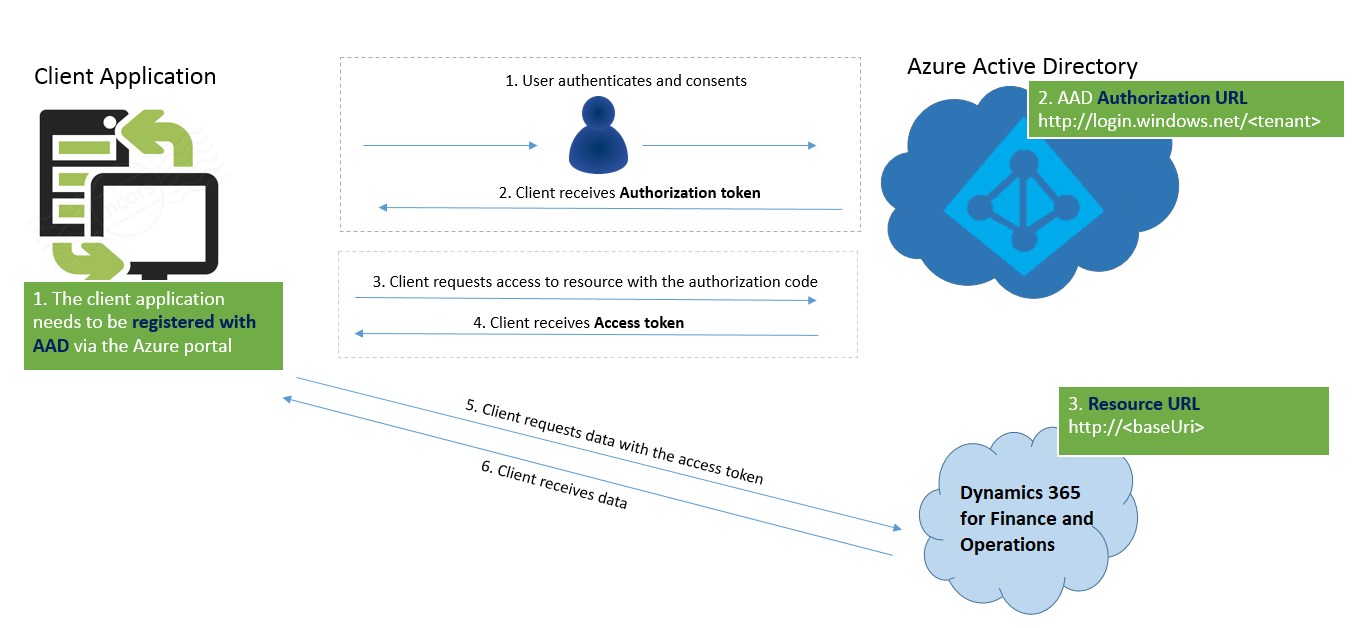
\includegraphics[width=1\textwidth]{img/aadAuthenticationArchitecture.png}
    \caption{D365FO authenticatie mbv Azure Active Directory}
\end{figure}
\section{Azure resources}
Aangezien alles gehost wordt op Azure, werden er ook een aantal Azure resources gebruikt. 

\subsection{D365FO implementatie}
Voor de Dynamics implementatie zelf worden er geen Azure resources gebruikt in termen van hosting of dergelijke. Wel is het zo dat een D365FO omgeving steeds op azure draait. In het geval van dit onderzoek draait D365FO lokaal op een developer Virtual Machine, die gehost staat op Azure. Dit zet MS echter allemaal klaar vanzelf. 

Ook werd er voor de authenticatie (zie later) gebruik gemaakt van het Azure AAD. Hiervoor werd een App Service aangemaakt in Azure: 

\begin{figure}[H]
    \centering
    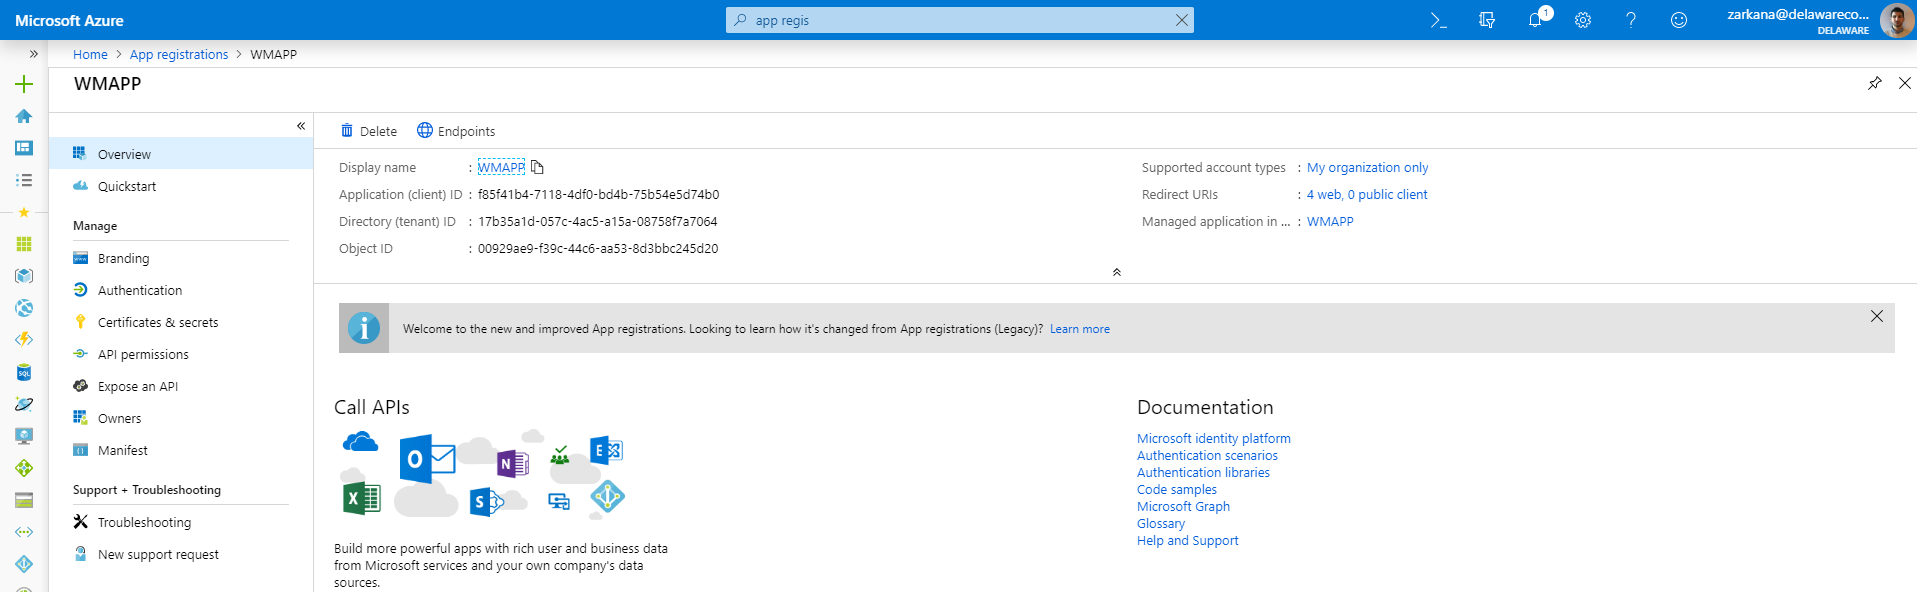
\includegraphics[width=1\textwidth]{img/appRegistrationD365fo.png}
    \caption{In Azure aangemaakt app service voor de authenticatie met D365FO vanuit externe apps}
\end{figure}

\subsection{Bot implementatie}

\subsection{Authenticatie applicatie}
Ook voor de authenticatie applicatie werden er resources aangemaakt in Azure. Dit om de applicatie te kunnen hosten, maar ook om inzichten te kunnen verwerven adhv Application Insights. Dit is een APM (Application Performance Management) service die gebruikt kan worden om live web applicaties te monitoren op vele gebieden zoals verkeer etc., maar ook is Application Insights geschikt om te troubleshooten wanneer er zich problemen voordoen. In onderstaande afbeelding vindt men screenshots terug vanuit Portal.azure.com: 

\begin{figure}[H]
    \centering
         \includegraphics*[width=1\textwidth]{img/ResourceAuthentication1.png}
        \caption{Azure resource voor de effectieve webhosting van de authenticatie app}
    \end{figure}
    \begin{figure}[H]
        \includegraphics*[width=1\textwidth]{img/ResourceAuthentication2.png}
        \caption{Azure resource voor de Application Insights gekoppeld aan de authenticatie app}
\end{figure}  

\section{Data model}
Binnen D365FO zullen custom klassen en methodes gebruikt worden bovenop de reeds bestaande. De reden hiervoor is om op efficiënte manier informatie te kunnen versturen in webrequests. Het gebruiken van de bestaande klassen in D365FO zou een vorm van overkill zijn, omdat deze heel veel data en andere informatie bevatten die niet relevant is voor het poc. Deze klassen zullen vervolgens geserialiseerd verstuurd worden als JSON-objecten. 

\subsection{Json 2 Csharp}
De in D365FO (X++) geïmplementeerde klassen zullen vervolgens ook nodig zijn in de authenticatie app (C\#). Dit zodat de geserialiseerde JSON objecten gedeserialiseerd kunnen worden in C\# objecten. Hiervoor kan men er voor kiezen om alles dubbel te programmeren, wat dus ook dubbel werk betekent. Een andere optie is echter om de JSON strings te gebruiken voor de conversie. Hier zijn verschillende sites en tools voor, waarvan Json2Csharp.com een voorbeeld is. 
In onderstaande afbeelding wordt geïllustreerd hoe dit in zijn werk gaat. De geserialiseerde JSON string kan integraal geplakt worden, waarna de tool automatisch C\# klassen zal creëren die op hun beurt slechts gekopieerd en geplakt moeten worden in een nieuwe lege C\# klasse.
\begin{figure}[H]
    \centering
    \includegraphics[width=1\textwidth]{img/json2Csharp.png}
    \caption{Json2Csharp voorbeeld}
\end{figure}

\section{UML}
Uiteraard werd er alvorens de poc gemaakt kon worden een klassendiagram opgesteld. Er werd gekozen om een eigen data model te ontwerpen en implementeren aangezien de reeds bestaande klasses in D365FO al een lange tijd meegaan, en veel onnodige informatie bevatten wat betreft de scope van dit onderzoek.\\De klassen die in onderstaande figuur staan opgelijst zijn grotendeels extensies van reeds bestaande klassen. Dit omdat het een business vereiste was dat de chatbot kon communiceren met de huidige D365FO omgeving. De extensies werden daarom enkel gemaakt zodat er geen onnodige informatie moest worden verstuurd in de requests, maar ook omdat de data die verstuurd werd terug gedeserialiseerd moet worden in een andere programmeertaal (\C#). Hiervoor werd JSON2Csharp gebruikt (zie 6.6.1). Als men er echter voor zou kiezen om de bestaande klassen in D365FO te serialiseren en te versturen in webrequests zou dit aanzienlijk meer geheugen en computing power vereisen daar de bestaande entiteiten in D365 van dermate omvang zijn (sommige zijn al meer dan 20 jaar oud!) dat dit ongetwijfeld een bottleneck zou betekenen wat betreft throughput van D365FO naar third-party apps. 
\begin{figure}[h!]
    \centering
    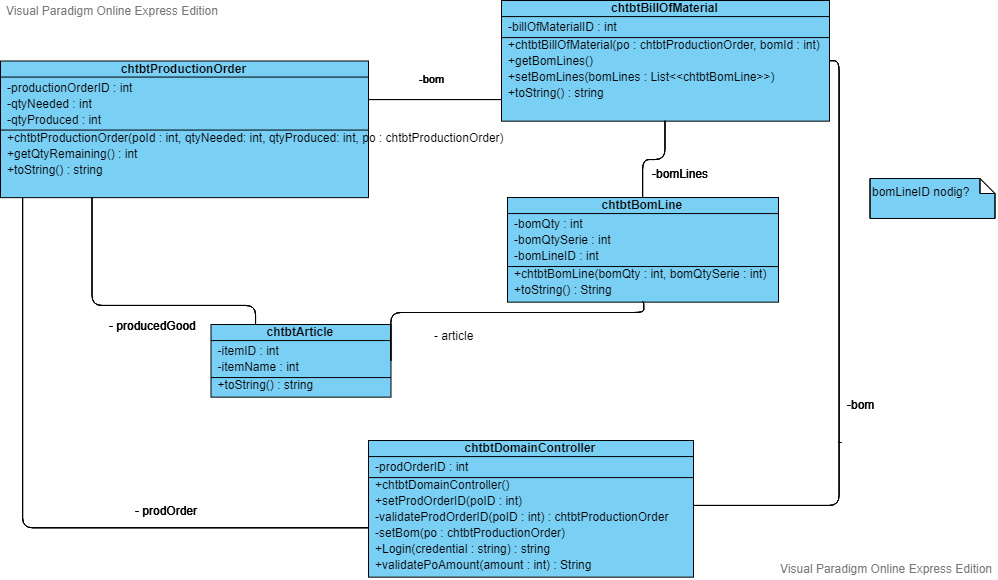
\includegraphics[width=1\textwidth]{img/Uml}
    \caption{UML voor de must-have functionaliteiten van het poc}
\end{figure}